\chapter{Резюме на глава 6: Уеб портал}
\label{webportal}

Под \href{http://openbiodiv.net}{openbiodiv.net} може да се стигне до основния портал, който дава достъп до ресурсите на OpenBiodiv. Този портал е разработен от Pensoft в подкрепа на OpenBiodiv и представя два визуални елемента на потребителя: лентата за търсене и списък с икони на приложения в долната част. Освен това, под \href {http://graph.openbiodiv.net}{{graph.openbiodiv.net}} (също достъпен от иконката SPARQL) може да се достигне работния плот OpenBiodiv за  на SPARQL.

Тези функции на потребителския интерфейс (UI) са предназначени да улеснят трите типа потребители на системата, които предвиждаме:

\begin{enumerate}
\item Основно ниво: използва лентата за търсене.
\item Ниво на специалист: използва приложения.
\item Power user: използва работната плот за SPARQL или R.
\end{enumerate}

\begin{figure}
\centering
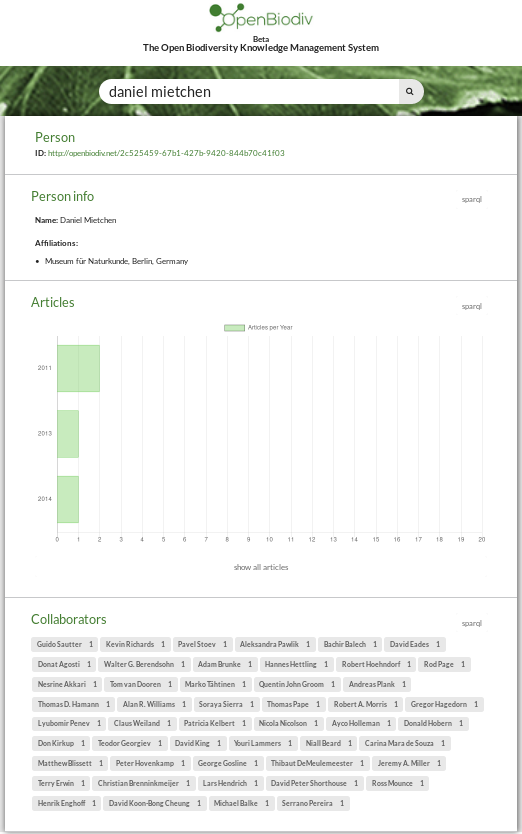
\includegraphics[width=\textwidth]{Figures/basic-level.png}
\decoRule
\caption{Илюстрация на основната употреба на OpenBiodiv за търсене на информация за човек.}
\label{fig:basic-level}
\end{figure}